\documentclass{article}
\usepackage{float}
\usepackage{hyperref}
\usepackage{graphicx} % Required for inserting images
\usepackage{booktabs}

\graphicspath{{../figures/figures_report_1/}}

\title{ANALYSIS OF COVID-19 CHEST X-RAYS: Report 1: Exploration, data visualization, and data pre-processing report}
\author{Saniya Arfin, Yvonne Breitenbach, Alexandru Buzgan}
\date{April 2025}

\begin{document}

\maketitle

\tableofcontents

\newpage 

\section{Introduction}

\subsection{{Context}}

Saniya: This project is very relevant to my translational oncology and biomedical research background. It directly involves the analysis of real patient data in the form of chest radiographs, a clinically significant modality often used in diagnostic workflows. The classification of COVID-19 and related lung pathologies through machine learning aligns well with my experience in biomarker discovery, cancer diagnostics, and data-driven decision support. The hands-on application of advanced machine learning algorithms, along with techniques for data preprocessing, bias detection, and model interpretability, further strengthens my skill set in translational bioinformatics, making this project both practically valuable and conceptually aligned with my future goals in medical AI.\\

\vspace{0.3cm}

Yvonne: As I have no background in medicine, biology or the analysis of medical data, the context of this project is completely new to me. Furthermore, I have no experience working with X-ray images or in image processing in general.
However, working on this project is very valuable to me as a meteorologist because meteorology also often works with image data, such as satellite images or radar images. In recent years, the use of machine learning and deep learning models has become more and more important in meteorology as in many industries. For example, to classify cloud types in satellite images and overall to improve the weather forecast. 
My goal is to combine what I will learn from the work on this project with my meteorological background to apply this in future jobs. \\

\vspace{0.3cm}

Alexandru:I chose this project because of my interest in image recognition. I have a background as a Software Engineer in the automotive industry, and the development of self-driving automobiles makes use of this type of technologies quite often. The skills I will acquire on this project will suit me in the projects that I hope to work on in the future. Image recognition and classification may hold the key to the future of autonomous vehicles, which will have to identify and classify possible obstacles on their path. Both supervised and unsupervised learning algorithms are key components of these technologies.
My goal is to add these skills to my previous experience and be better prepared for the technologies of tomorrow. 
\newpage
\subsection{Objectives}
\vspace{0.3cm}
\begin{itemize}
    \item Early detection of COVID-19 from X-rays 
    \item Importance of radiology in pandemics
    \item Compare COVID-19 with other diseases (e. g., viral pneumonia)
    \item Real-world implications (e. g., hospital triage, AI for diagnostics)
\end{itemize}

\vspace{0.5cm}
\subsection{Goals}
\vspace{0.3cm}
\underline{Identifying the problem}\\

Supervised learning: Here we try to predict the target variable (dependent): COVID, Normal, Viral Pneumonia, Lung Opacity using supervised learning. Since we are looking to predict a qualitative variable it is a classification problem. To achieve this, the following steps must be carried out:
\begin{itemize}
    \item Classify chest X-ray images
    \item Understand dataset distribution
    \item Identify class imbalance, noise, or biases
    \item Prepare data for a ML/DL model
\end{itemize}

\newpage 

\section{Understanding and manipulation of data}

\subsection{Framework}

\paragraph{Dataset}\
We obtained COVID-19 Radiography Dataset.zip (777 MB) from Kaggle (https://www.kaggle.com/datasets/tawsifurrahman/covid19-radiography-database). This dataset is open access.



\paragraph{Dataset Description}
The dataset includes X-ray images of lungs and their corresponding masks. Table \ref{tab:xray_lung_masks} shows the distribution of the X-ray images and the lung masks by class. In all four classes there are as many X-ray images as lung masks.

% Requires: \usepackage{booktabs}
\begin{table}[h]
    \centering
    \begin{tabular}{|l|c|c|}
        \hline
        \toprule
        \textbf{class} & \textbf{number of X-ray images} & \textbf{number of lung masks} \\
        \hline
        \midrule
        Normal & 10192 & 10192 \\
        \hline
        Lung Opacity & 6012 & 6012 \\
        \hline
        COVID & 3616 & 3616 \\
        \hline
        Viral Pneumonia & 1345 & 1345 \\
        \hline
        \bottomrule
    \end{tabular}
    \caption{Distribution of X-ray images and lung masks by class}
    \label{tab:xray_lung_masks}
\end{table}

The normal class contains X-ray images of healthy lungs. The other three classes contain X-ray images of diseased lungs. The diseases are divided into COVID-19, viral pneumonia and lung opacity (non-COVID lung infections). 


\paragraph{Metadata}
Additionally to the X-ray images and lung masks there are four metadata files available on the Kaggle website.

\begin{itemize}
    \item COVID.metadata.xlsx
    \item Lung\_Opacity.metadata.xlsx
    \item Normal.metadata.xlsx
    \item Viral Pneumonia.metadata.xlsx
    \end{itemize}

These metadata files contain additional information, e. g. the size of the images and their source. 

\subsection{Pre-processing and feature engineering}

\vspace{0.5cm}

\subsubsection{Exploratory Data Analysis (EDA)} \label{sec:EDA}
\vspace{0.5cm}

\underline{Class Distribution}\\
\\
As already shown in table \ref{tab:xray_lung_masks} the four classes contain different numbers of images. Figure \ref{fig:class-dist} illustrates the distribution of images and masks in the different classes. Almost half of all images/ masks (48.2 \%) belong to the "Normal" class. Second most images/ masks are in the "Lung Opacity" class (28.4 \%), followed by the "COVID" class (17.1 \%). The "Viral Pneumonia" class contains the least images/ masks (6.4 \%).

\vspace{0.3cm}

\begin{figure}[h!] % the [h!] helps force it "here"
    \centering
    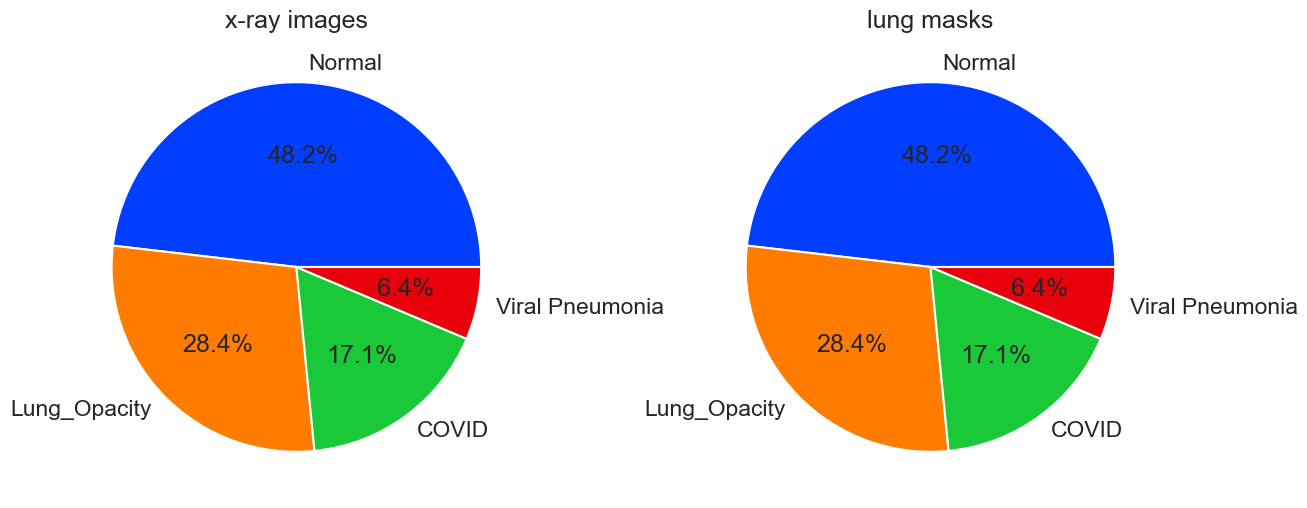
\includegraphics[width=1.0\linewidth]{classes.png}
    \caption{Precentage of X-ray images and lung masks by class}
    \label{fig:class-dist}
\end{figure}

\vspace{0.5cm}

\noindent \underline{Image Visualization}\\
\\
In order to get an idea of the X-ray images five examples of each of the four classes are shown in figure \ref{fig:example_xray_classes}.


\begin{figure}[h!] % the [h!] helps force it "here"
    \centering
    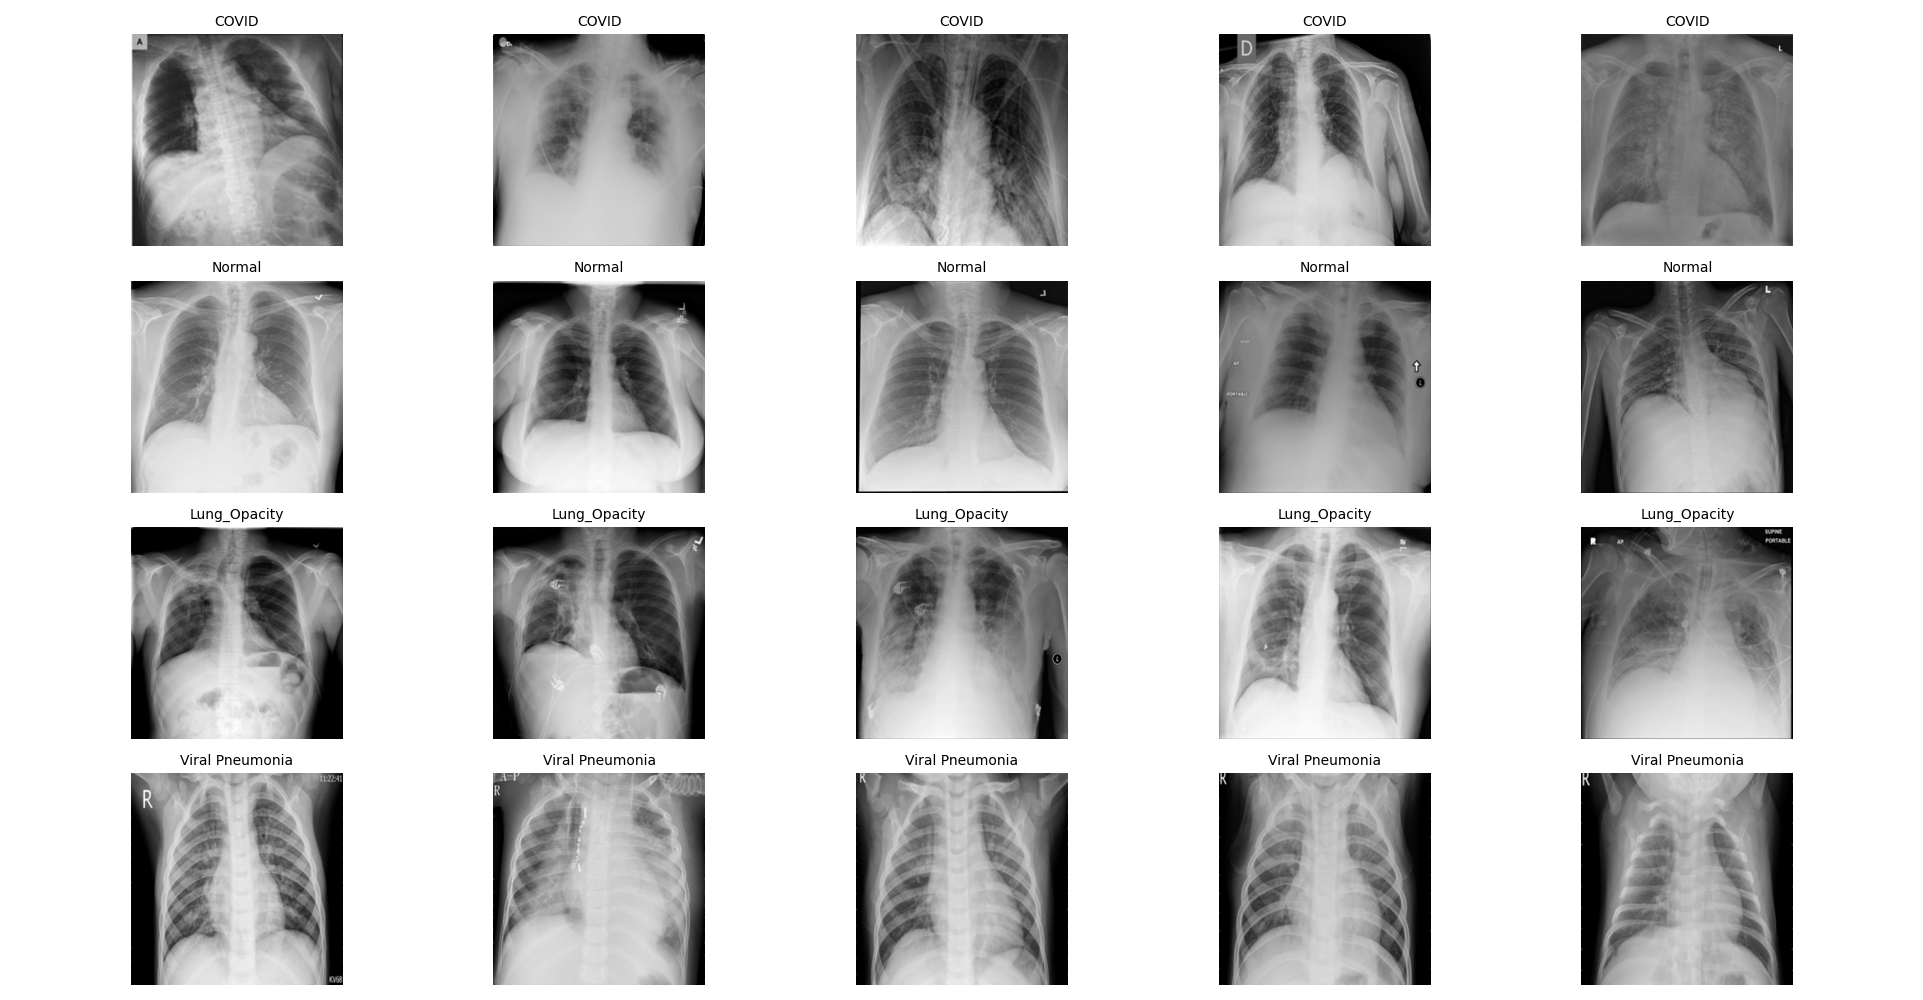
\includegraphics[width=1.0\linewidth]{20figures_grid.png}
    \caption{Examples of X-ray images of the four classes}
    \label{fig:example_xray_classes}
\end{figure}

\vspace{0.5cm}

\noindent \underline{Image Size Distribution and Type of Image}\\
\\
In the four files with metadata the size of each image is given. We first analyzed the image sizes from these metadata files and found out that all the images have the same size: 256 x 256 pixel. \\
As a next step we opened each X-ray image and the lung masks with Python and determined their sizes. The read-out image sizes are summarized in table \ref{tab:iamges_sizes}. All the lung masks have a size of 256 x 256 x 3 pixel. The first two dimensions are the same as specified in the metadata files. But the masks have additionally a third dimension, which indicates that they aren't saved as grayscale images. \\
The analysis showed that the size of the X-ray images in the first two dimensions is 299 x 299 pixels and therefore different from the size of the lung masks. Therefore we conclude that the lung masks have to be resized before matching them with the X-ray images. \\
Besides that, the table \ref{tab:iamges_sizes} shows that most of the X-ray images (21025) have only two dimensions and therefore are grayscale images. But there are 140 X-ray images that have three dimensions and thus aren't grayscale images. These 140 RGB images belong to the class "Viral Pneumonia". Figure \ref{fig:modes_viral_pneumonia} shows the proportion of RGB- and grayscale images in the class "Viral Pneumonia". These RGB-images should be converted into grayscale images before using them for modeling. \\

\begin{table}[h]
    \centering
    \begin{tabular}{|c|c|c|}
        \hline
        \textbf{Image size} & \textbf{Number of X-ray images} & \textbf{Number of lung masks} \\ \hline
        299 x 299 x 3 & 140 &  \\ \hline
        299 x 299 & 21025 &  \\ \hline \hline
        256 x 256 x 3 &  & 21165 \\ \hline
    \end{tabular}
    \caption{Size of X-ray images and lung masks}
    \label{tab:iamges_sizes}
\end{table}

\begin{figure}[h!] % the [h!] helps force it "here"
    \centering
    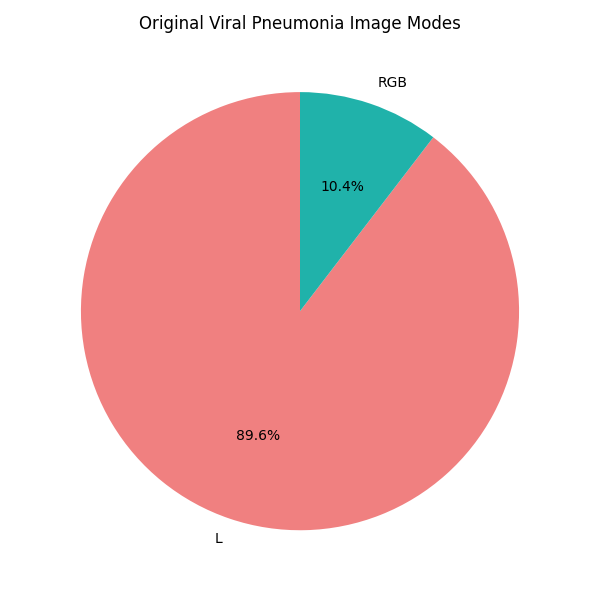
\includegraphics[width=0.5\linewidth]{rgb vs L.png}
    \caption{Proportion of RGB- and L modes in the class "Viral Pneumonia".}
    \label{fig:modes_viral_pneumonia}
\end{figure}

\vspace{0.3cm}\newpage
              
\noindent \underline{File format consistency} \\
\\
We confirmed format consistency to avoid read errors, and we observed all images were in PNG format as shown in Fig. \ref{fig:image-format}.

\vspace{0.3cm}

\begin{figure}[h!]% the [h!] helps force it "here"
    \centering
    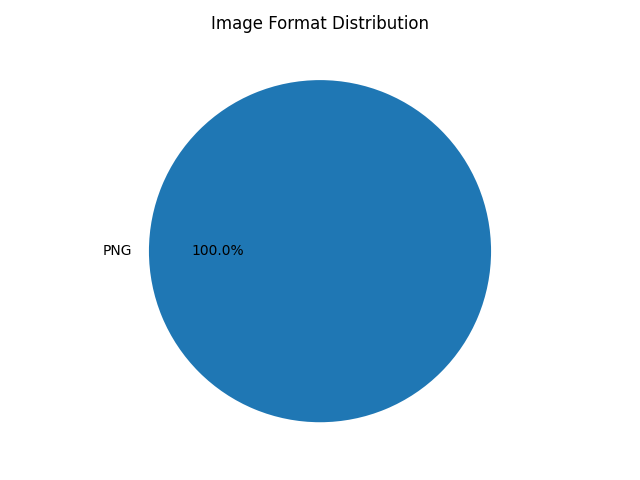
\includegraphics[width=0.7\linewidth]{image_format_distribution.png}
    \caption{Image format distribution}
    \label{fig:image-format}
\end{figure}   

\vspace{0.3cm}
\newpage
\noindent \underline{ Class Proportion by Source URL} \\
\\
To identify potential dataset bias by image source, we plotted a stacked bar chart of image count by class and URL source, figure  \ref{fig:distr_source_url}.  This figure and table \ref{tab:image-sources} show that the X-ray images come from eight different sources. Most of the images come from the source https://www.kaggle.com/c/rsna-pneumonia-detection-challenge/data. \\
Further investigation shows that all images of the "Lung Opacity" class and most images of the "Normal" class come from this source. The remaining part of the "Normal" classes images and all images of the class "Viral Pneumonia" are from the source https://www.kaggle.com/paultimothymooney/chest-xray-pneumonia. The images of the "COVID" class come from six other sources, but most of them from https://bimcv.cipf.es/bimcv-projects/bimcv-covid19/\#1590858128006-9e640421-6711. \\
Further analysis has to be done to investigate if the images from different sources are somehow different. 


\begin{figure}[h!] % the [h!] helps force it "here"
    \raggedright
    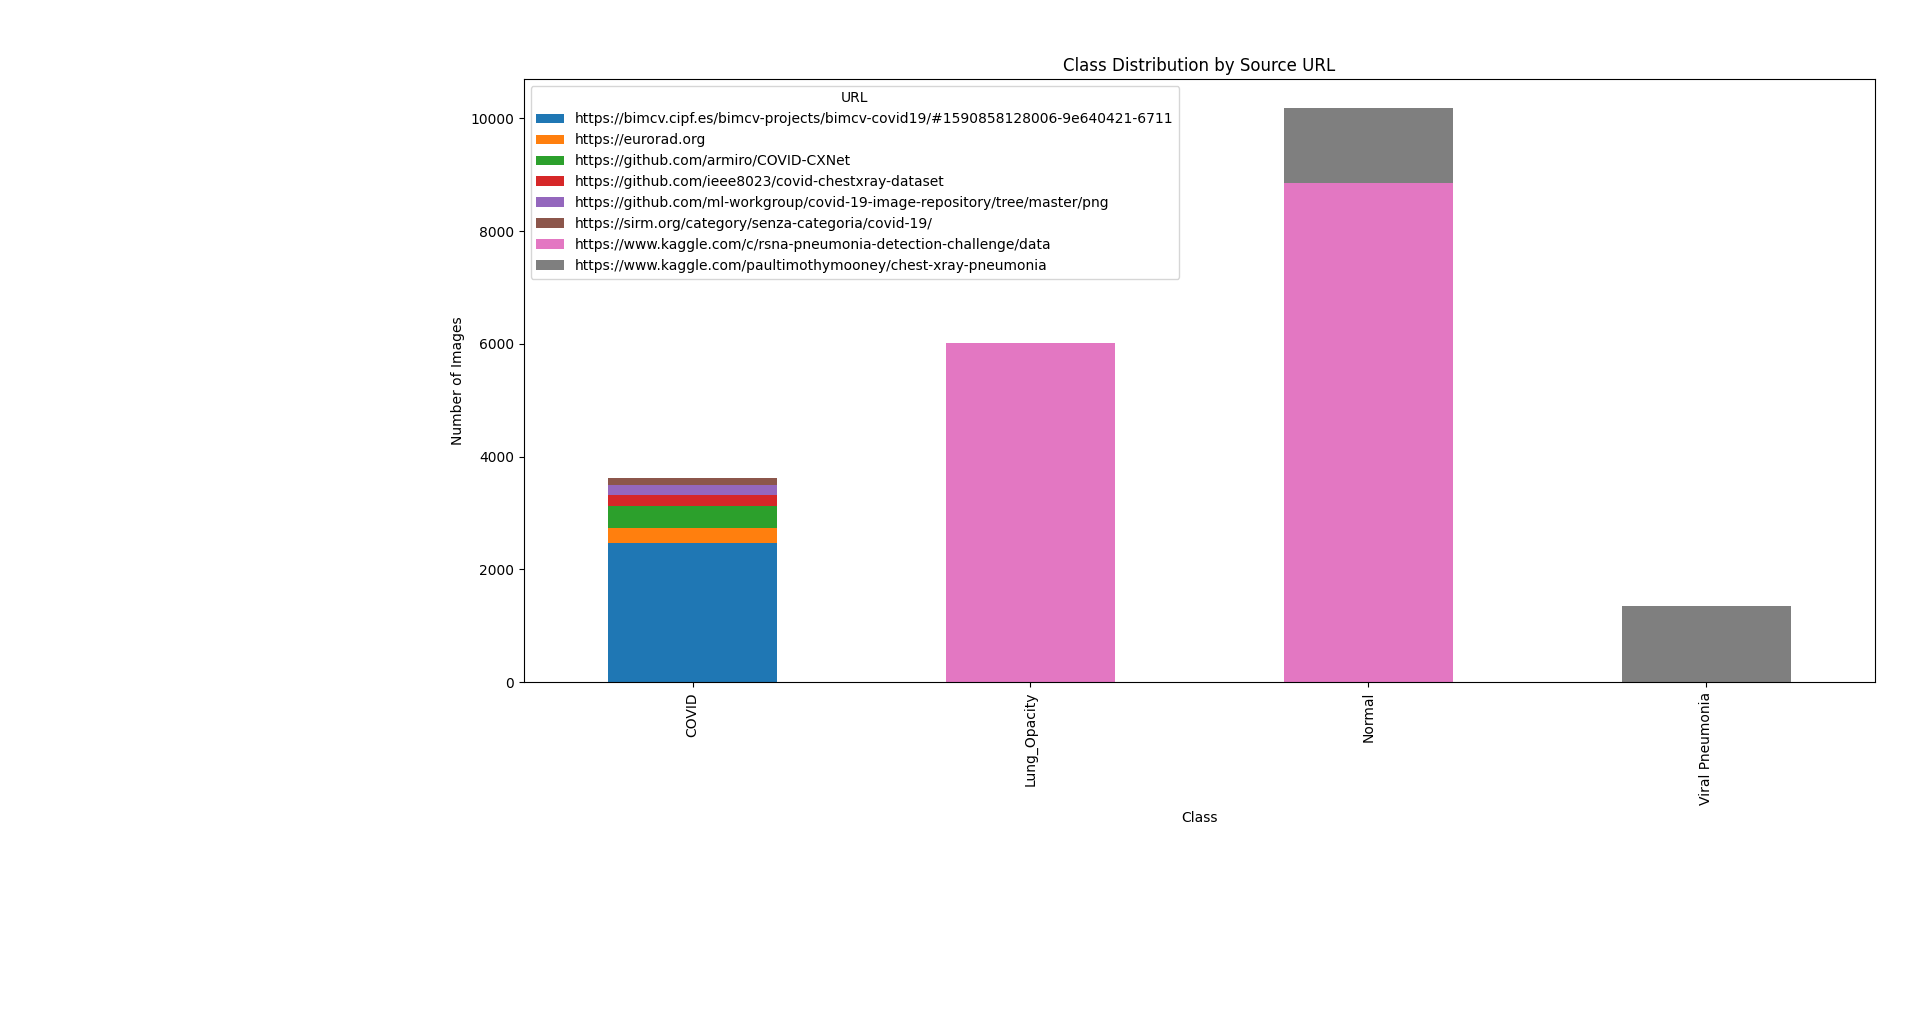
\includegraphics[width=1.0\linewidth]{class_distrbution_by_source_url.png}
    \caption{Class Distribution by source url}
    \label{fig:distr_source_url}
\end{figure}


\begin{table}[h!]
    \centering
    \begin{tabular}{|l|p{8cm}|r|}
        \hline
        \textbf{Label} & \textbf{URL} & \textbf{Count} \\
        \hline
        COVID & \url{https://bimcv.cipf.es/bimcv-projects/bimcv-covid19/#1590858128006-9e640421-6711} & 2474 \\
        \cline{2-3}
        & \url{https://eurorad.org} & 258 \\
        \cline{2-3}
        & \url{https://github.com/armiro/COVID-CXNet} & 400 \\
        \cline{2-3}
        & \url{https://github.com/ieee8023/covid-chestxray-dataset} & 182 \\
        \cline{2-3}
        & \url{https://github.com/ml-workgroup/covid-19-image-repository/tree/master/png} & 183 \\
        \cline{2-3}
        & \url{https://sirm.org/category/senza-categoria/covid-19/} & 119 \\
        \hline
        Lung\_Opacity & \url{https://www.kaggle.com/c/rsna-pneumonia-detection-challenge/data} & 6012 \\
        \hline
        Normal & \url{https://www.kaggle.com/c/rsna-pneumonia-detection-challenge/data} & 8851 \\
        \cline{2-3}
        & \url{https://www.kaggle.com/paultimothymooney/chest-xray-pneumonia} & 1341 \\
        \hline
        Viral Pneumonia & \url{https://www.kaggle.com/paultimothymooney/chest-xray-pneumonia} & 1345 \\
        \hline
    \end{tabular}
    \caption{Image source URLs and corresponding image counts for each label.}
    \label{tab:image-sources}
\end{table}




\newpage

\vspace{0.5 cm}

\subsubsection{Exploratory Data Visualizations}\

\vspace{0.3 cm}

We created class-wise smoothed Kernel Density Estimate (KDE) plots\\

\begin{itemize}
\item for mean pixel intensities and
\item for standard deviations (std) of pixel intensities.
\end{itemize}


\vspace{0.5cm}

\begin{figure}[h!] % the [h!] helps force it "here"
    \centering
    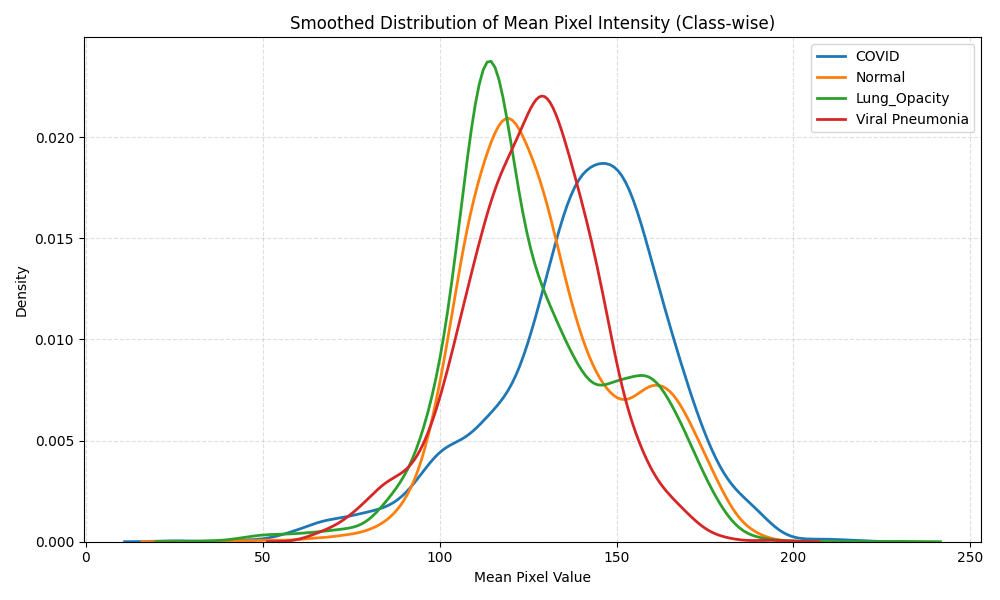
\includegraphics[width=0.5\linewidth]{KDE.Pixelintensity.png}
    \caption{Distribution of mean pixel intensity by Image classes}
    \label{fig:distr_mean_pixel_class}
\end{figure}
    
\paragraph{}
\underline{Inference:}\
Different classes show distinct mean intensity patterns. COVID images tend to be brighter on average, potentially due to artifacts or progression patterns, while Lung Opacity images are darker.

\vspace{0.5cm}

\begin{figure}[h!] % the [h!] helps force it "here"
    \centering
    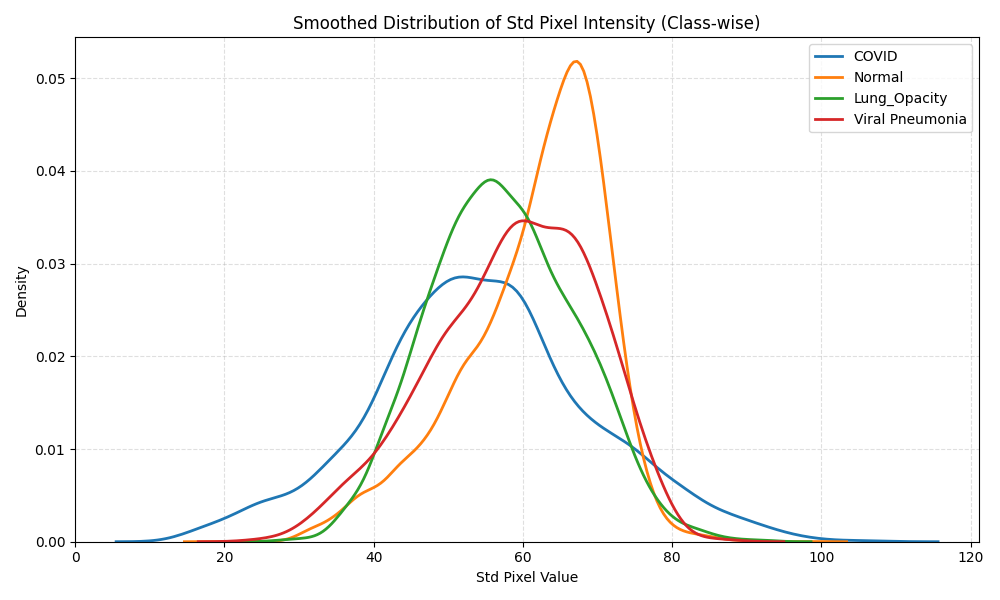
\includegraphics[width=0.5\linewidth]{distribution_of_std_pixel_all.png}
    \caption{Distribution of standard deviation of pixel intensity by Image classes}
    \label{fig:distr_std_pixel_class}
\end{figure}

\vspace{0.5cm}

\underline{Inference:}\
COVID images have higher variability in pixel intensity, possibly due to complex lung patterns like patchy opacities. Normal images are consistent and smooth.

\vspace{0.5cm}

Additionally, we created sourcewise smoothed Kernel Density Estimate (KDE) plots to identify source bias\\
\begin{itemize}
\item for mean pixel intensities and
\item for standard deviations (std) of pixel intensities.
\end{itemize}


\begin{figure}[h!] % the [h!] helps force it "here"
    \centering
    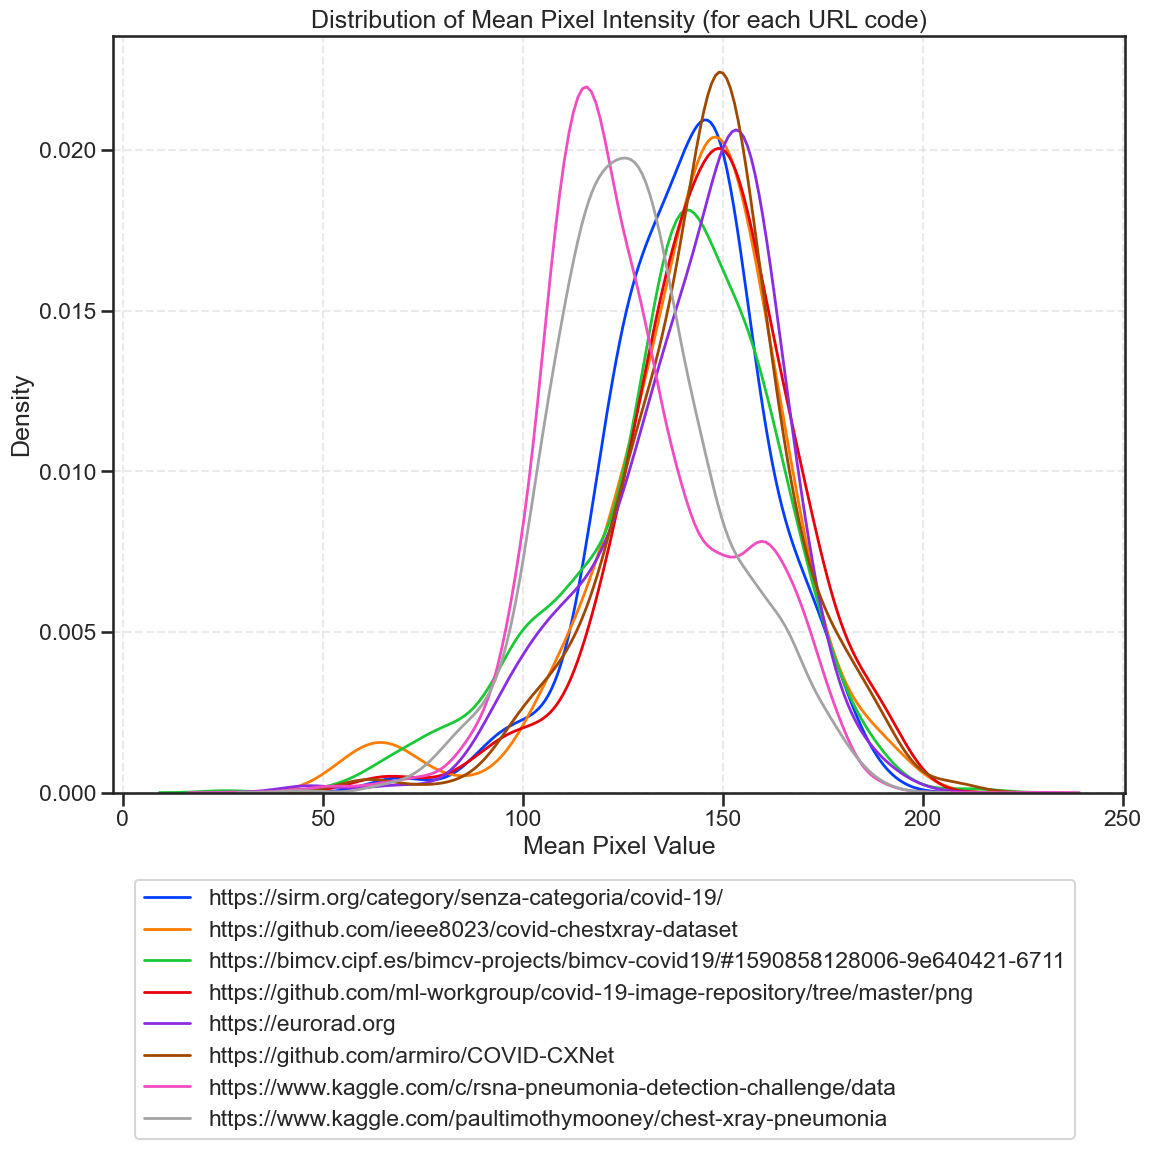
\includegraphics[width=0.5\linewidth]{mean_pixel_sources.png}
    \caption{Distribution of mean of pixel intensities of the X-ray images depending on the different sources}
    \label{fig:distr_mean_pixel_source}
\end{figure}
\begin{figure}[h!] % the [h!] helps force it "here"
    \centering
    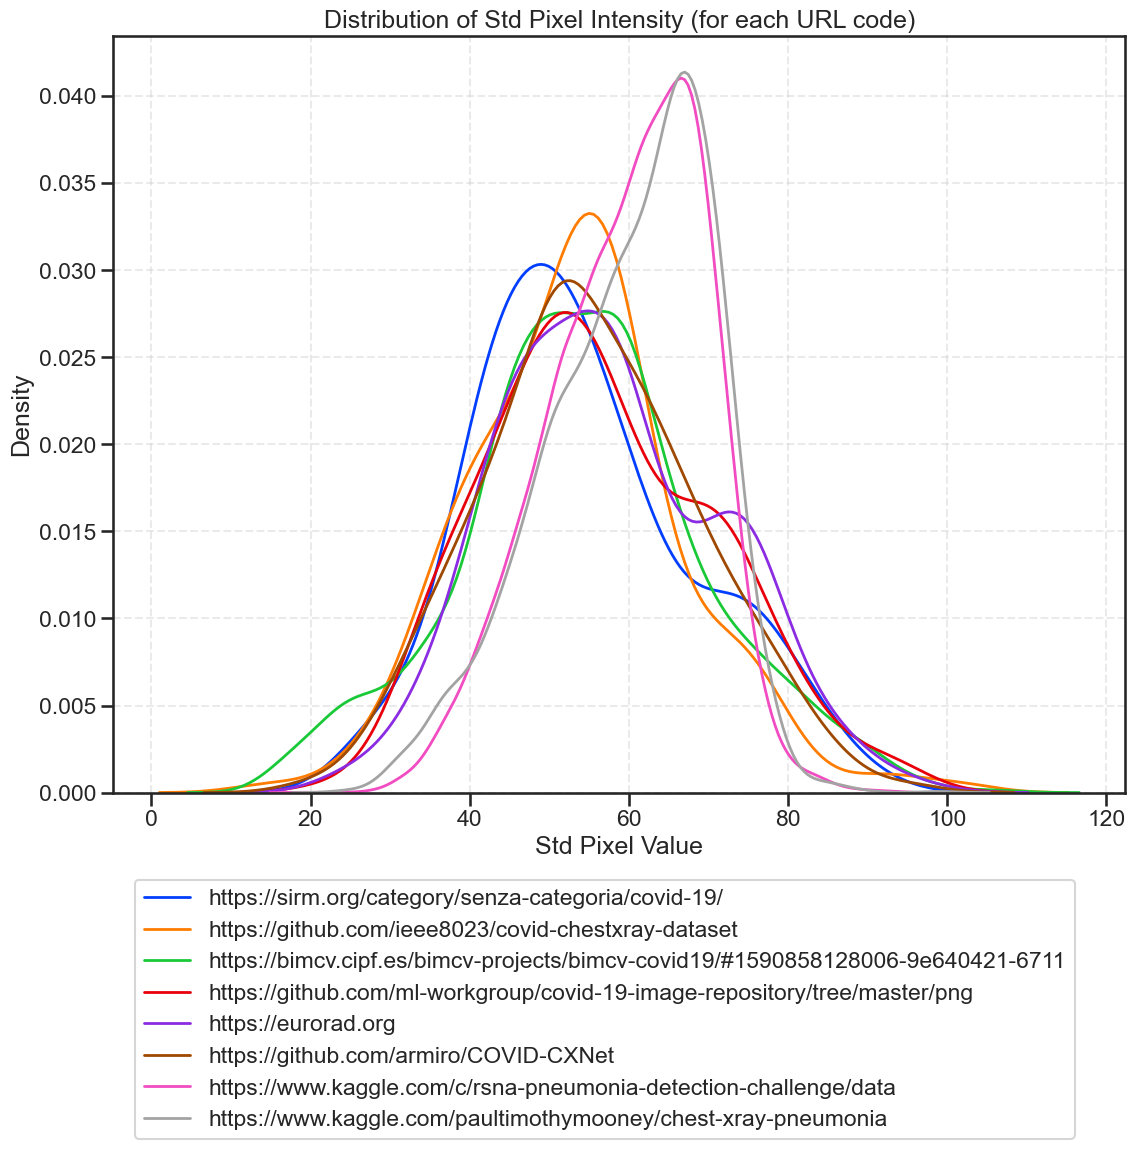
\includegraphics[width=0.5\linewidth]{std_pixel_sources.png}
    \caption{Distribution of standard deviation of pixel intensities of the X-ray images depending on the different sources}
    \label{fig:distr_std_pixel_source}
\end{figure}

\newpage
\underline{Inference:}\
Images from https://www.kaggle.com/paultimothymooney/chest-xray-pneumonia and
https://www.kaggle.com/paultimothymooney/chest-xray-pneumonia have different mean and std pixel intensities in comparison to the images from other sources.

On exploration of viral pneumonia images metadata we observed different image modes(figure \ref{fig:modes_viral_pneumonia}). This may be responsible for the higher variance (std) in RGB (due to color channels) as observed in figure \ref{fig:distr_std_pixel_source}. Inconsistent image modes create hidden discrepancies in data, therefore we try to fix this in the next steps.

\vspace{0.3cm}

\subsubsection{Mask Adjustment}\
As already described in chapter \ref{sec:EDA} we found out that the lung masks have not the same size as the X-ray images. The X-ray images have 299 x 299 pixel and the masks are smaller with only 256 x 256 pixel. Therefore the size of the masks have to be adjusted before one can overlay them with the X-ray images. We tried three different methods. 

The first method we tried out, was to expand the masks by adding some black areas to the masks so that their sizes is the same as the images. We tried to add black areas to the right side and below the masks. Besides, we tried to add black areas to the left side and above the masks. 
The second method we tried out, was a simple resizing of the masks to 299 x 299 pixel by using the resize-function of the OpenCV Python library. As interpolation method we used  “cv2.INTER\_CUBIC”.


\vspace{0.3cm}

\begin{figure}[h!]% the [h!] helps force it "here"
    \centering
    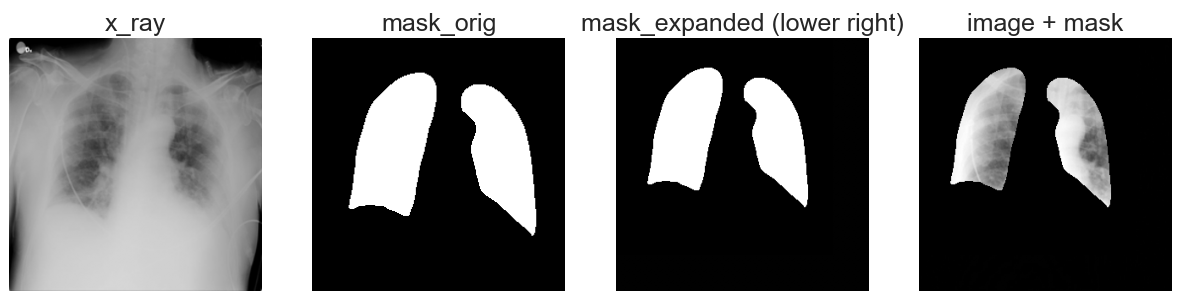
\includegraphics[width=1\linewidth]{lung_mask_report_lr.png}
    \caption{Modifying the lung mask by adding black areas to the right of the mask and below.}
    \label{fig:lung_mask_lr}
\end{figure}   


\begin{figure}[h!]% the [h!] helps force it "here"
    \centering
    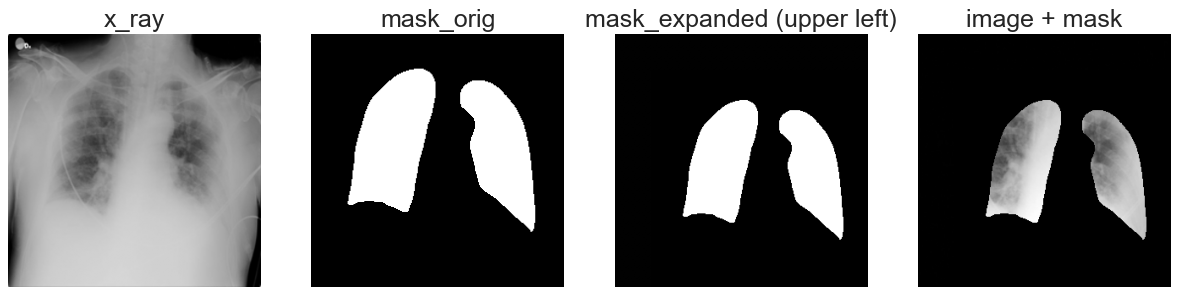
\includegraphics[width=1\linewidth]{lung_mask_report_ul.png}
    \caption{Modifying the lung mask by adding black areas to the left of the mask and above.}
    \label{fig:lung_mask_ul}
\end{figure}   


\begin{figure}[h!]% the [h!] helps force it "here"
    \centering
    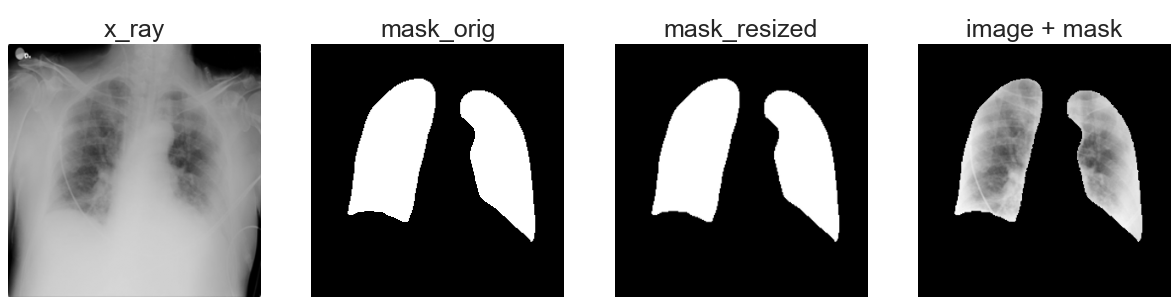
\includegraphics[width=1\linewidth]{lung_mask_report_resize.png}
    \caption{Modifying the lung mask by resizing them with OpenCV.}
    \label{fig:lung_mask_resize}
\end{figure}   

\vspace{0.3cm}

\noindent \underline{Inference:}\\
\\
Figures \ref{fig:lung_mask_lr}, \ref{fig:lung_mask_ul} and \ref{fig:lung_mask_resize} show  (from left to right) the X-ray image, the corresponding lung mask not modified, the modified lung mask and the modified lung mask added to the X-ray image. The mask which is resized with OpenCV fits best to the area where the lung is located in the X-ray image. This can be seen in detail in the overlay of some resized masks and X-ray images in figure \ref{fig:overlay_masks_images}.

\vspace{0.3cm}

\begin{figure}[h!]% the [h!] helps force it "here"
    \centering
    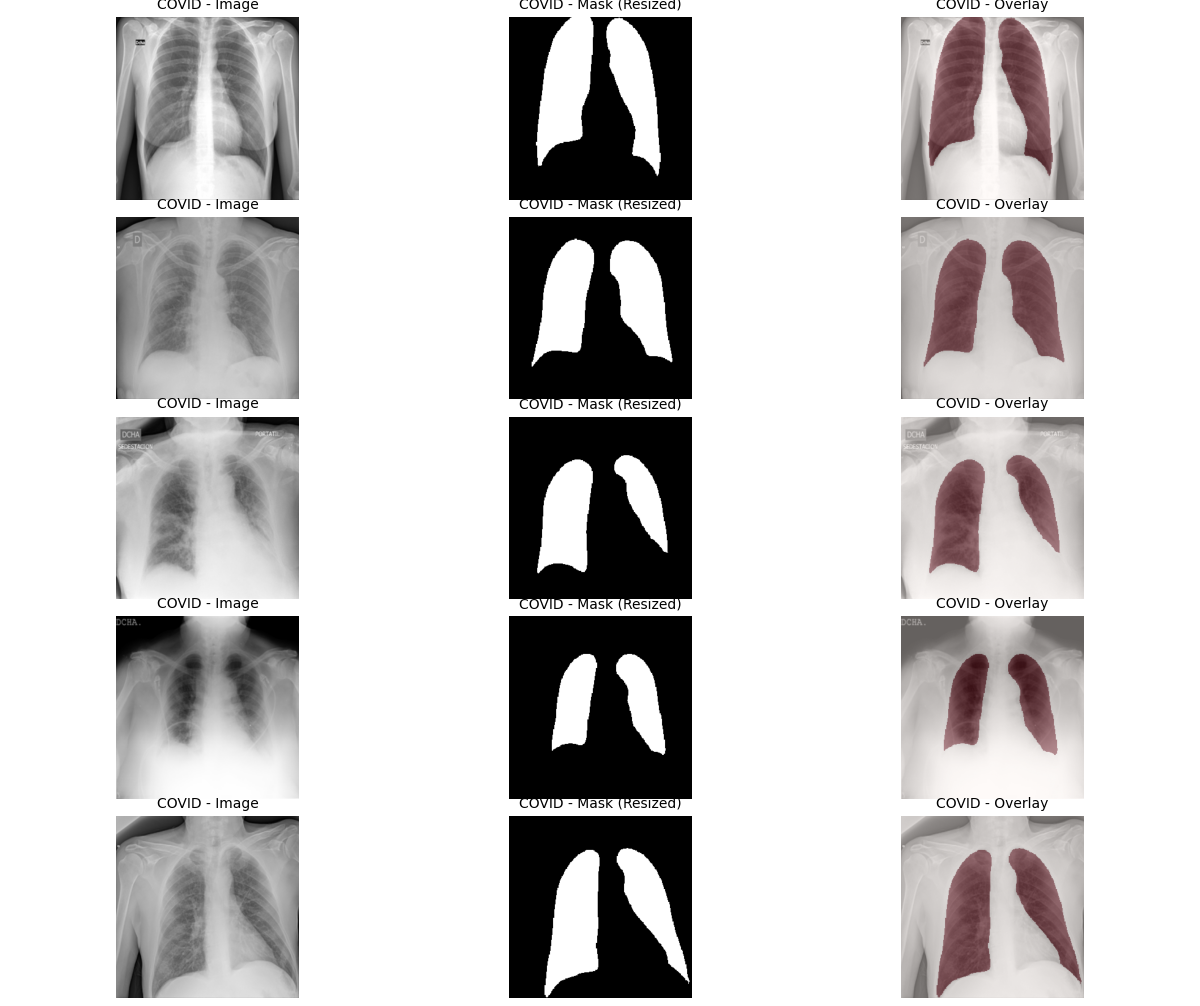
\includegraphics[width=1\linewidth]{overlay_masks_images.png}
    \caption{Overlay of resized masks and X-ray images.}
    \label{fig:overlay_masks_images}
\end{figure}   

\vspace{0.3cm}

\vspace{0.5cm}



\vspace{0.3cm}

\subsubsection{Preprocessing Pipeline}\

\vspace{0.5cm}

To minimize source-related bias and standardize image quality across the dataset, we applied the following preprocessing steps:

\vspace{0.3cm}

1. Removed source bias:

\begin{itemize}
    \item Grayscale Conversion (L-channel): All images were converted to grayscale using OpenCV (RGB conversion to L) to eliminate color-related variability and focus solely on intensity information.
    \item Contrast Enhancement with CLAHE: Applied CLAHE to help standardize the contrast across images, reducing the impact of varying imaging conditions. For example, images taken with different machines or in different settings may have varying brightness and contrast levels. Local enhancement ensures greater uniformity between images.
       
    \item Lung Region Isolation: Mask resizing (from 256*256 to 299*299) and applying the binary mask to the image after CLAHE (Contrast Limited Adaptive Histogram Equalization) processing, we ensured that only the lung regions are enhanced and normalized, while irrelevant areas like the background are not affected.

    \begin{figure}[h!] % the [h!] helps force it "here"
        \centering
        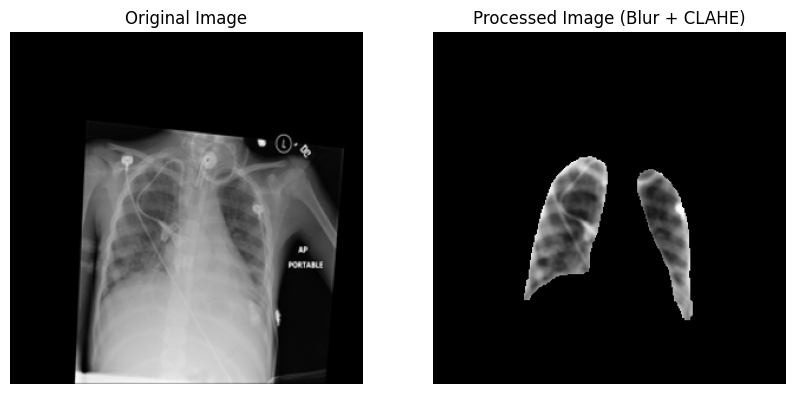
\includegraphics[width=0.5\linewidth]{ORIGINAL+PROCESSED IMAGE.png}
        \caption{Original X-ray image (left) and filtered X-ray image with applied mask (right)}
        \label{fig:enter-label}
    \end{figure}
     
    \item Pixel Value Normalization: Since some images from one source are brighter or darker than those from another, normalizing the images ensures that they all lie within the same range, preventing models from learning biased patterns based on intensity differences. The images are converted to numpy arrays and stored as.npz files for fast loading during training and evaluation.

\end{itemize}
\newpage
\subsection{Visualizations Post Processsing}

\begin{figure}[h!] % the [h!] helps force it "here"
    \centering
    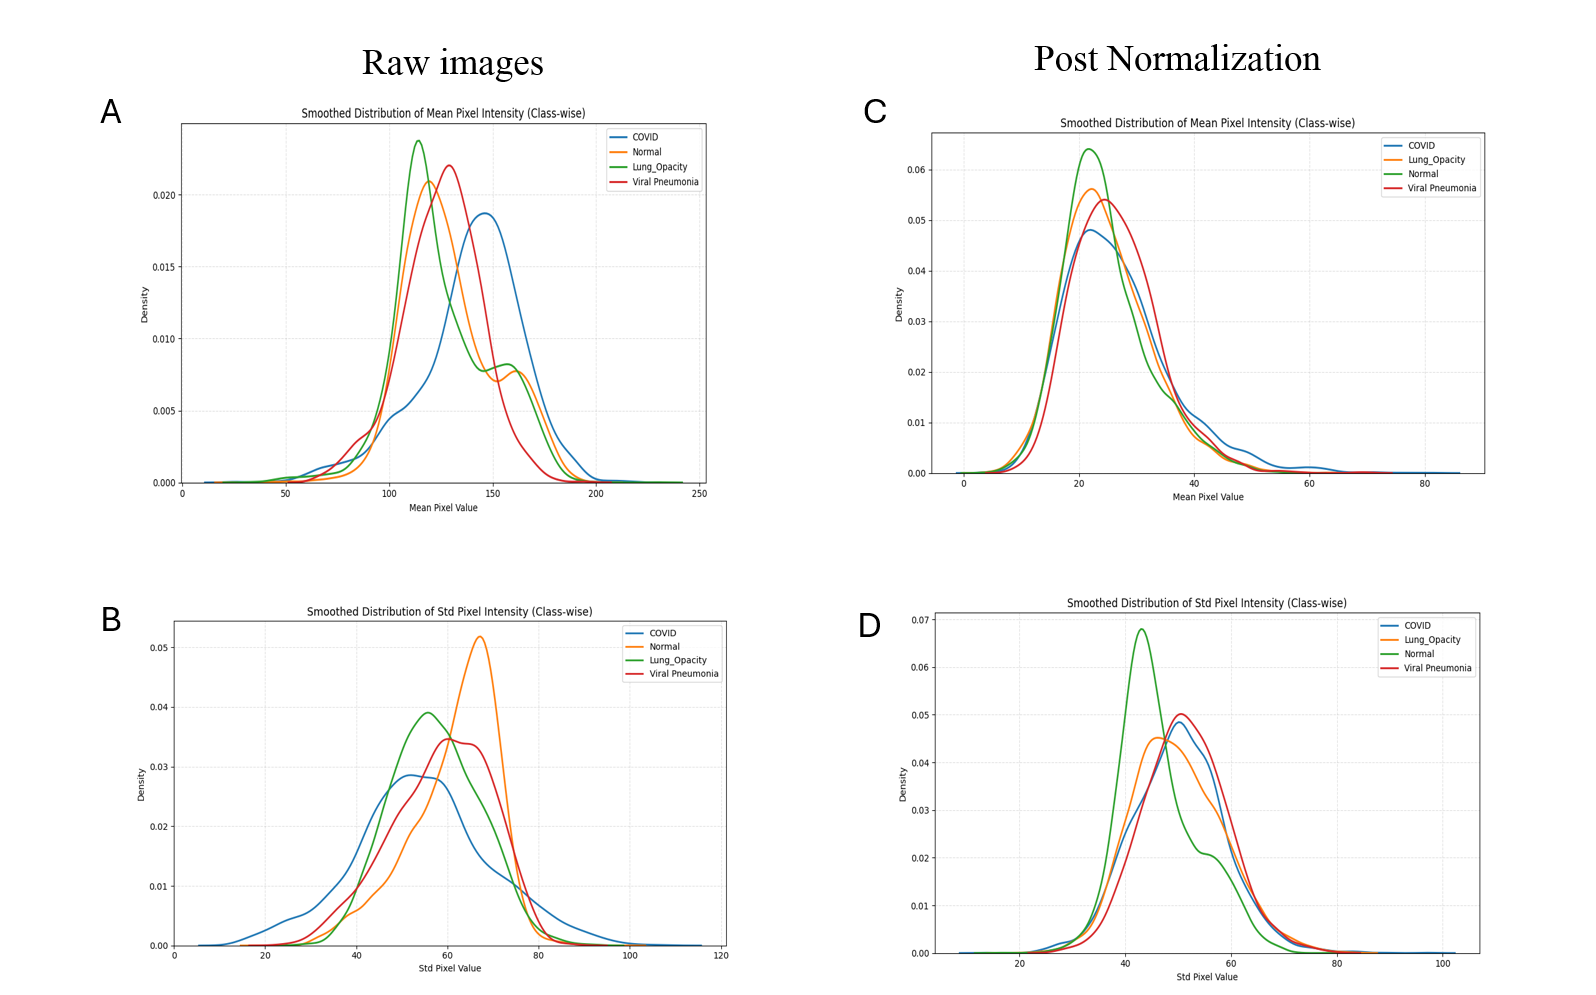
\includegraphics[width=1.0\linewidth]{Screenshot 2025-04-21 223200.png}
    \caption{Distribution of mean and std of pixel intensities of the X-ray images before and after normalization by classes}
    \label{fig:KDE_pre_post_normalization_class}
\end{figure}
\vspace{0.3cm}
\underline{Inference:}\

In images A and B in figure \ref{fig:KDE_pre_post_normalization_class} we observe that raw images (left panels) have significantly different mean and standard deviation values of pixel intensities across the four classes: COVID, Normal, Lung Opacity, and Viral Pneumonia. This variation reflects inherent differences in image acquisition conditions or dataset characteristics, which could introduce bias into any machine learning model by enabling it to learn spurious class-specific brightness or contrast cues. After normalization, figure  \ref{fig:KDE_pre_post_normalization_class} (C and D) (right panels), these distributions become considerably more aligned. Both mean and standard deviation values show tighter and more overlapping density curves, indicating that normalization effectively reduces class-specific pixel-level discrepancies. This helps ensure that the model focuses on medically relevant features rather than superficial intensity differences, thus improving generalization and fairness.

\vspace{0.3cm}
\newpage
\begin{figure}[h!] % the [h!] helps force it "here"
    \centering
    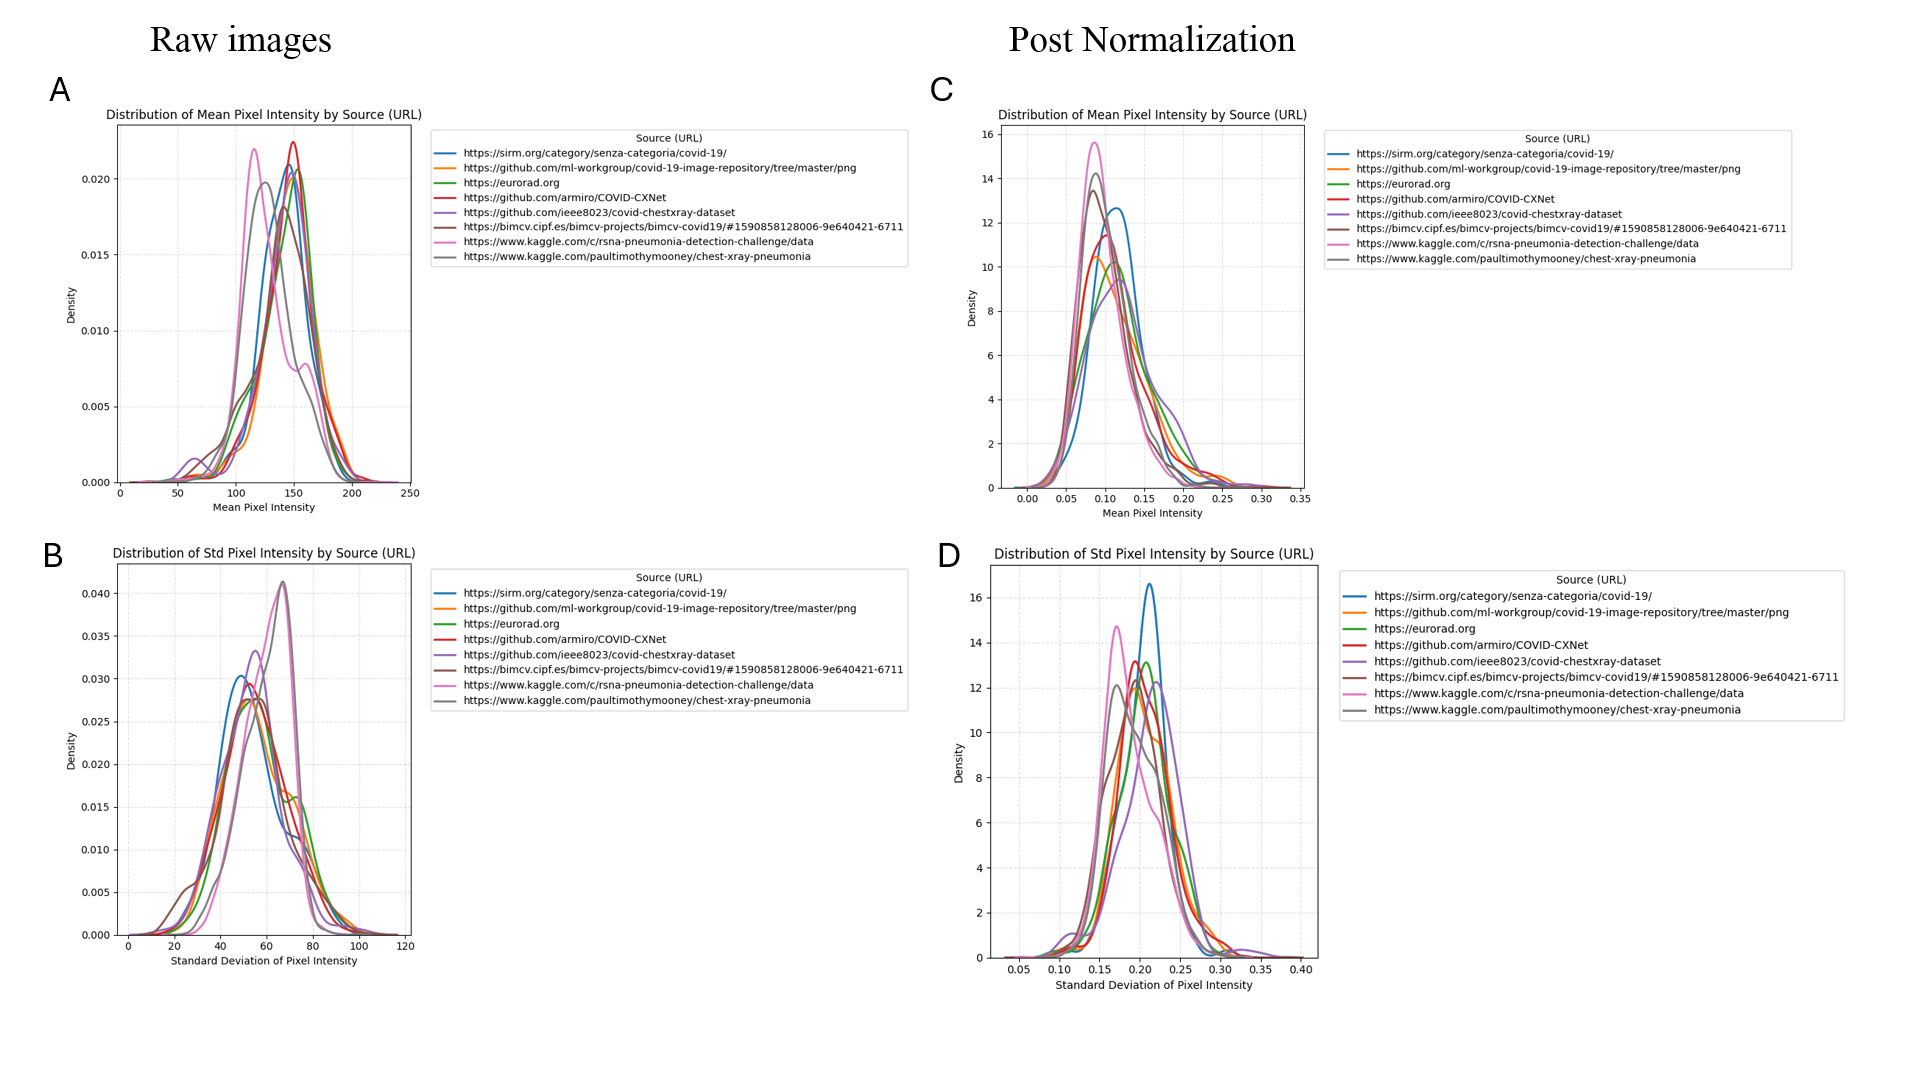
\includegraphics[width=1.0\linewidth]{Screenshot 2025-04-21 223207.png}
    \caption{Distribution of mean and std of pixel intensities of the X-ray images before and after normalization by sources}
    \label{fig:KDE_pre_post_normalization_URL}
\end{figure}

\vspace{0.3cm}

\underline{Inference:}\
In figure \ref{fig:KDE_pre_post_normalization_URL}, a similar trend is analyzed but from a source-wise perspective. Each line in the plots represents data from a different image source or URL. The raw images in figure \ref{fig:KDE_pre_post_normalization_URL} (A and B) (left panel) again show substantial variation in both mean and standard deviation of pixel intensities across sources, suggesting a strong presence of domain shift — a critical issue when training models on aggregated datasets from different institutions or platforms. Such differences can hinder a model’s performance on unseen data if not addressed. Post normalization (right panels), the pixel intensity distributions across all sources become much more consistent. This is a vital step in preparing the data for robust, real-world model deployment.

\vspace{0.3cm}

\newpage
\newpage

\subsection{Next Steps}\

\begin{itemize}
\item Label Encoding
Convert categorical class labels (e.g., COVID, Normal, Pneumonia, Lung Opacity) into numerical format for compatibility with machine learning algorithms.
\item Dataset Splitting
Partition the dataset into training, validation, and test subsets to enable robust model evaluation and prevent data leakage.
\item Address Class Imbalance
Since the distribution between the classes is not balanced (for example Viral Pneumonia images are far less numerous than the Normal images) we have to address this problem before the training stage.
Appropriate strategies will be applied, such as:

Class weighting during model training

Oversampling/undersampling

Data augmentation for minority classes

This ensures the model does not become biased toward the majority classes and maintains fair performance across all categories.


\end{itemize}

\end{document}
